\documentclass[11pt]{article}
\usepackage[hmargin={1in},vmargin={1in,1in}]{geometry}   
\geometry{letterpaper}       
\usepackage{color,graphicx}
\usepackage{covington}
\usepackage{setspace}
\usepackage{amsmath}
\usepackage{amssymb}
\usepackage{varioref}
\usepackage{textcomp}
\usepackage{textcomp}
\usepackage{mflogo}
\usepackage{wasysym}
\usepackage{pstricks, pst-plot, pst-node, pst-tree, colortab}
\usepackage{qtree}
\usepackage[normalem]{ulem}
\usepackage{hyperref}
\usepackage{natbib}
\renewcommand{\bibsection}{}
\usepackage{booktabs}
\usepackage{linguex}

\newcommand{\HRule}{\rule{\linewidth}{0.25mm}}

\usepackage{fancyhdr} % This should be set AFTER setting up the page geometry
\pagestyle{fancy} % options: empty , plain , fancy
\lhead{{Investigating Italian adjective ordering}}\chead{}\rhead{}
\renewcommand{\headrulewidth}{.5pt}
\lfoot{}\cfoot{\thepage}\rfoot{}
%\renewcommand{\footrulewidth}{.3pt}
\newcommand{\txtp}{\textipa}
\renewcommand{\rm}{\textrm}
\newcommand{\sem}[1]{\mbox{$[\![$#1$]\!]$}}
\newcommand{\lam}{$\lambda$}
\newcommand{\lan}{$\langle$}
\newcommand{\ran}{$\rangle$}

\newcommand{\bex}{\begin{exe}}
	\newcommand{\eex}{\end{exe}}

\newcommand{\bit}{\begin{itemize}}
	\newcommand{\eit}{\end{itemize}}

\newcommand{\ben}{\begin{xlist}}
	\newcommand{\een}{\end{xlist}}

\newcommand{\type}[1]{\ensuremath{\left \langle #1 \right \rangle }}

\renewcommand\theenumi {\alph{enumi}}
\renewcommand\theenumii {\alph{enumii}}
\renewcommand\labelenumi {\theenumi. }
\renewcommand\labelenumii {\theenumii.}
\labelformat{enumi}{(\theenumi)}
\labelformat{enumii}{(\theenumi\theenumii)}
\newcounter{saveenumi}

\renewcommand{\labelitemii}{\textbf{$\circ$}}

\renewcommand{\firstrefdash}{}

%\linespread{1.5}
%\thispagestyle{empty}

\title{Investigating Italian adjective ordering}
\author{Greg Scontras, Rita Manzini, Greta Mazzaggio}

\begin{document}
	
\maketitle
		
		
Speakers have robust preferences for the relative order of adjectives when multiple adjectives modify a noun (e.g., \emph{big blue box} vs.~\emph{blue big box}); these preferences have been well-documented in English, together with a host of unrelated languages (see \citealp{scontras2023}, for an overview). Importantly, the preferences observed in an AAN language like English appear as the mirror image in NAA languages like Arabic. We investigate adjective ordering in a language with both pre- and postnominal adjectives: Italian. While ANA templates have received a good deal of discussion in the theoretical literature on adjective ordering (e.g., \citealp{cinque1994,cinque2010}), quantitative behavioral data are lacking. 		
		
\section{Background}

In many languages, the very same adjectives can be pre- or postnominal, with no obvious interpretive consequences, see Italian \Next[a]. However, while practically all adjectives can be postnominal, certain adjectival classes are claimed to be barred from prenominal position, see \Next[b] \citep{giorgilongobardi1991, cinque1994}. \cite{cinque1994} crucially observes that the restriction in (1b) interacts with the classical typological and theoretical issue of the internal order of adjectives, as determined by classes such as color, shape, size \citep{sproatshih1991}. Lower adjectives in the typological sequence are normally postnominal, while higher adjectives can be pre- or postnominal.         

\ex. \ag.	Ha          comprato una nuova macchina / macchina nuova\\
S/he.has bought      a     new   car           \emph{/} car           new\\
\bg.     	Ha         comprato una   macchina giapponese / *giapponese macchina\\
s/he.has bought     a    	car   	    Japanese    \emph{/} Japanese      car\\
`S/he bought a Japanese car.'


\cite{cinque1994,cinque2010} proposes a commonly-adopted solution, namely that the prenominal order is base generated, respecting a semantically determined order, (2a), while postnominal order depends on movement of N to an intermediate position in the adjectival sequence.  \cite{cinque2010}, modifying \cite{cinque1994}, accepts that Romance postnominal order mirrors prenominal order, being produced by so-called ``roll-up'' movement. For instance, in (2b), NP moves to Spec of A$_{nationality}$ and the constituent so created moves to Spec of A$_{color}$.

\ex.   	
\a.     	\ldots [$_\textsc{ap}$ A$_{quality}$ [$_\textsc{ap}$ A$_{size}$  [$_\textsc{ap}$ A$_{shape}$ [$_\textsc{ap}$ A$_{color}$ [$_\textsc{ap}$ A$_{nationality}$  [$_\textsc{np}$ N \ldots
\b.     	\ldots [$_\textsc{ap}$      [$_\textsc{ap}$ NP  [$_{\textsc{a}'}$ A$_{nationality}$]]  \quad   	[$_{\textsc{a}'}$ A$_{color}$    

However, predictions about postnominal adjectives are not as sharp as (2) would suggest, given that any postnominal A for \cite{cinque2010} could be a reduced relative clause (RR). RR As are deemed to follow direct modification As (as a result of their relative height of attachment and of further obligatory roll-up movement). A direct modification order A$_1$--A$_2$ could be reversed if A$_1$ is a RR---or if both are RRs. The question, then, is what the ordering preferences are in ANA and NAA sequences in Italian, and whether we observe the flexibility predicted by the RR analysis in both cases. If RR structure is available as \citeauthor{cinque2010} claims, and both ANA and NAA sequences are derived from the same underlying AAN structure, then we expect similar flexibility in ANA and NAA orderings because any postnominal A could have RR syntax. If the RR analysis is unavailable, then we should observe a well-articulated hierarchy of ordering preferences in both ANA and NAA sequences, with the NAA template inverting the ordering observed in the ANA template as the result of roll-up movement. As the theory currently stands, we do not expect flexibility in one template but not in the other.
		
		

\section{Experiments}

We ran an Italian version of the ordering preferences experiment from \cite{scontrasetal2017adjectives}. The original English experiment tested ordering preferences for 26 adjectives from seven different semantic classes, randomly paired with ten different nouns (either food or furniture). The Italian materials appear in Table \ref{materials}; where possible, Italian materials are direct translations of the English materials from \citeauthor{scontrasetal2017adjectives}

On each trial, participants encountered a multi-adjective nominal formed by randomly pairing two adjectives and a noun from the materials in Table \ref{materials}, with the constraint that the two adjectives could not come from the same semantic class. Participants adjusted a slider to indicate which order of the adjectives sounded more natural; Figure \ref{example-trial} shows an example trial.


\begin{table}[htb]
	\caption{Adjectives and nouns used to form multi-adjective nominals in the Italian ordering preferences experiments.}
	\label{materials}
	\vspace{5pt}
	\centering
	\begin{tabular}{lll|lll}
		\toprule
		adjective & translation & class & 	adjective & translation & class  \\ \hline
		rosso	&	red		&	color		&	francese	&	French	& nationality\\
		giallo	&	yellow	& 	color		&	tedesco		&	German	& nationality\\
		verde	&	green	& 	color		&	liscio		&	smooth	& texture\\
		blu		&	blue	& 	color		&	duro		&	hard	& texture\\
		viola	& 	purple	& 	color		&	morbido		&	soft	& texture\\
		marrone	& 	brown	&  	color		&	vecchio		&	old		& age\\
		grande	& 	big		& 	size		&	nuovo		&	new		& age\\
		piccolo	& 	small	& 	size		&	marcio		&	rotten	& age\\
		gigantesco & huge	&	size		&	fresco		&	fresh	& age\\
		minuscolo & tiny	&	size		&	fantastico	&	wonderful & quality\\
		corto	&	short	&	size		&	cattivo		&	bad		& quality\\
		lungo	&	long	&	size		&	rotondo		& 	round	& shape\\	
		polacco &	Polish	&	nationality	&	quadrato	&	square	& shape\\ \bottomrule \toprule
		noun 	& translation & class		&	noun		&	translation & class \\ \hline
		mela	&	apple	&	food		&	sedia		&	chair	& furniture \\
		banana	&	banana	&	food		&	divano		&	sofa	& furniture \\
		carota	&	carrot	&	food		&	ventilatore	&	fan		& furniture \\
		formaggio &	cheese	&	food		&	televisore	&	television & furniture \\
		pomodoro &	tomato	&	food		&	scrivania	&	desk	& furniture \\ \bottomrule
	\end{tabular}
\end{table}


\begin{figure}[tb]
	\centering
	\fbox{
\includegraphics[width=5in]{example-trial.eps}}
	\caption{Example AAN trial.}
	\label{example-trial}
	\end{figure}

\subsection{Experiment 1: Within-subjects design}

On each trial, the multi-adjective nominal appeared randomly in one of three possible templates: AAN (as in Figure \ref{example-trial}), ANA, or NAA.

We recruited 120 participants via Prolific.com; we restricted our sample to people who indicated that they were raised monolingually speaking Italian. Of the 120 participants recruited, 108 indicated only Italian as the language spoken at home when they were children; we include the data from these 108 participants in the results reported below.

For each adjective, we calculated an average preferred-position measure, which represents how strongly that adjective is preferred in the linearly-first position; Figure \ref{results} plots these preferred-distance measures grouped by adjective semantic class. We find the most clearly-articulated preferences in the ANA template; moreover, the hierarchy observed in the ANA template largely matches that observed for English and other languages. 

In the AAN template, we find the weakest preferences, owing presumably to the fact that some of our adjectives have been claimed to be obligatorily post-nominal, which means that neither AAN order sounded natural. \cite{scontrasetal2017adjectives} found with English that cases where neither order sounded natural yielded chance-level ratings. 

The biggest surprise comes from the NAA template, where the preferred linear order of adjectives represents a weak mirror image of the ANA template. If the ANA template arises via movement from an underlyingly NAA structure, we might expect to find similarly-strong preferences for both templates. We wondered whether the weaker preferences for the NAA template arose because ANA is the preferred template, such that both NAA orders sound degraded relative to their ANA counterparts; this worry is heightened by the fact that participants encountered all three templates over the course of the experiment, thereby increasing the salience of the ANA template as an alternative to NAA.  

\begin{figure}[htb]
	\centering
	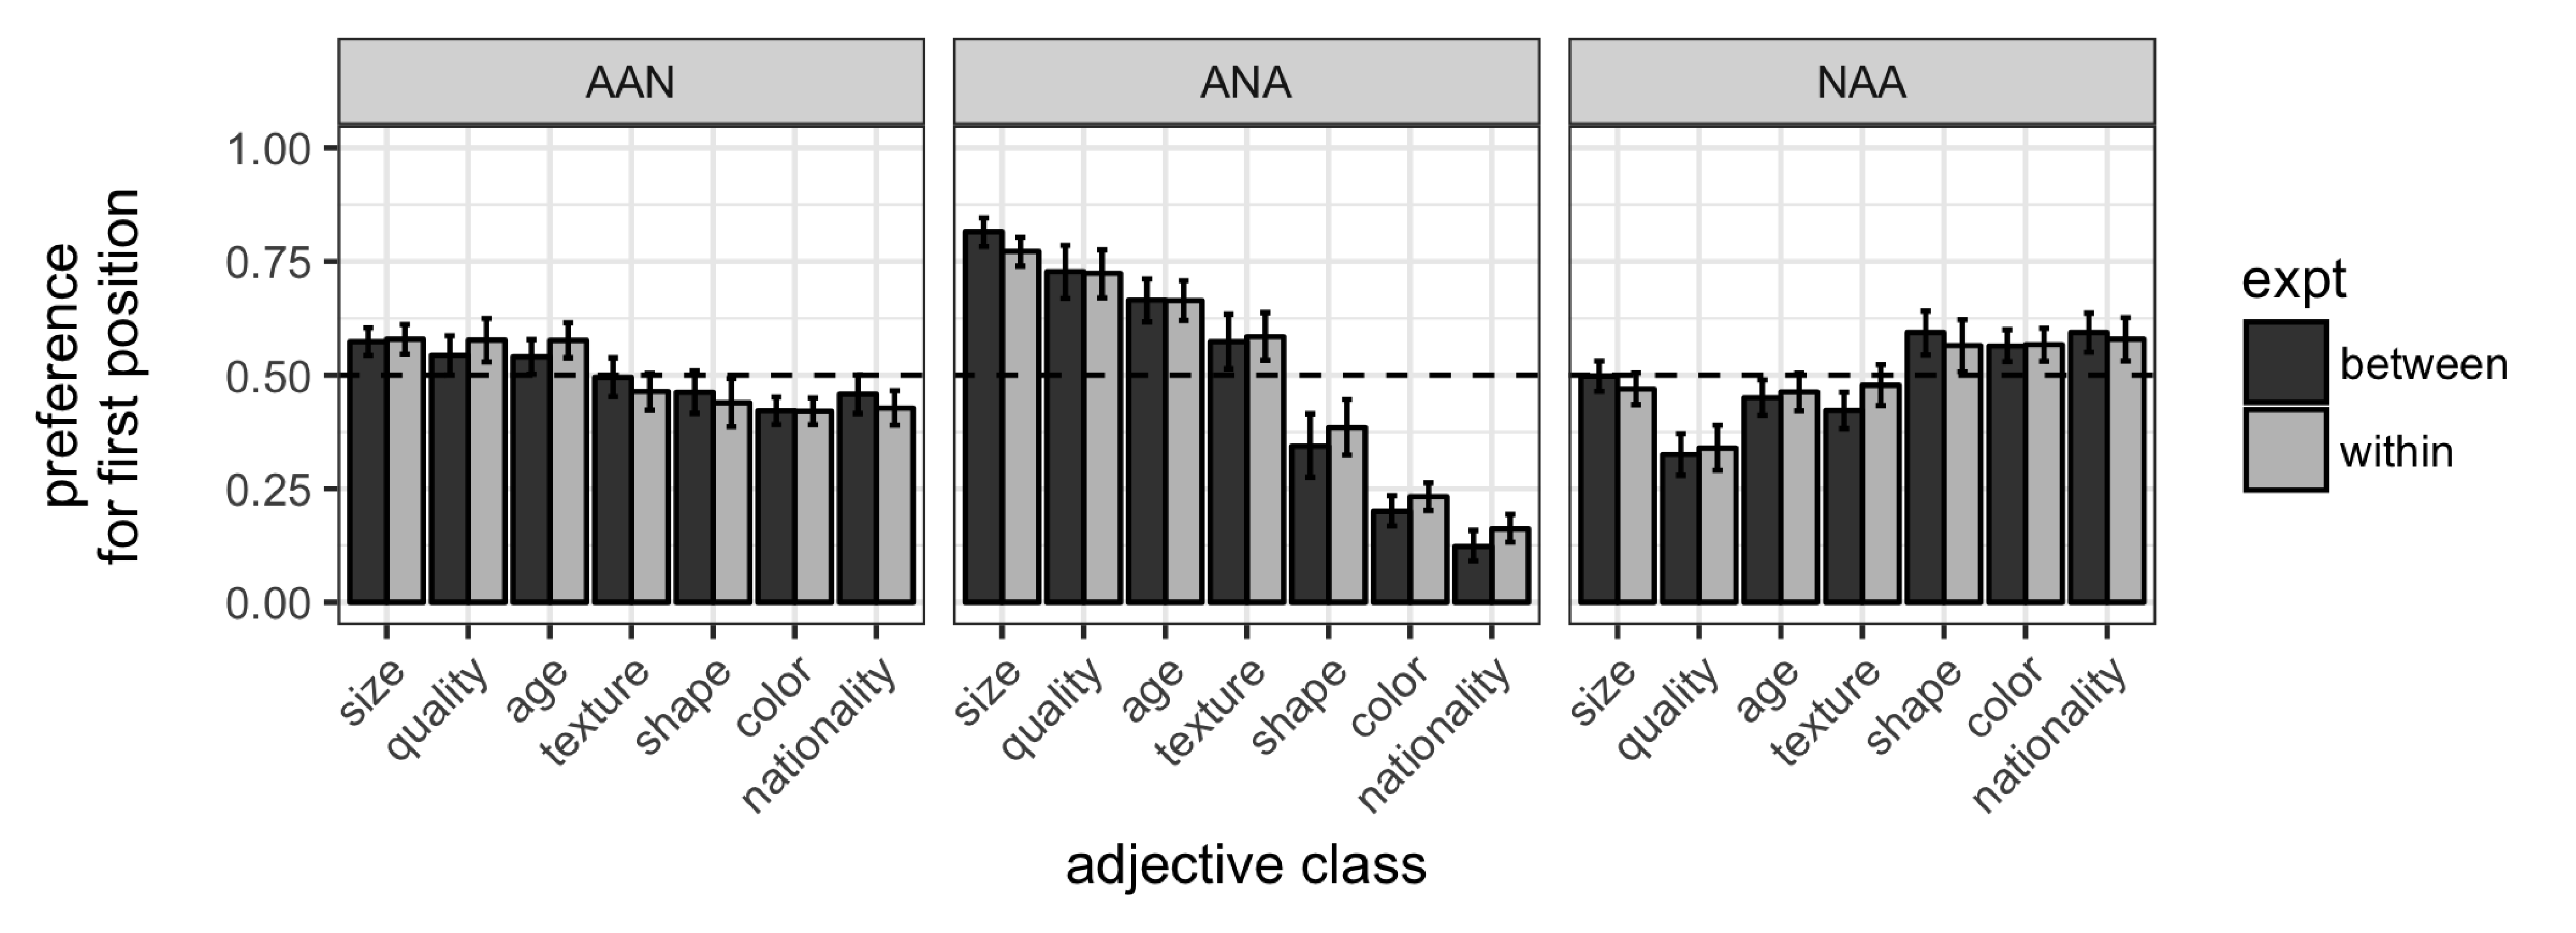
\includegraphics[width=\textwidth]{class_distance_combined.eps}
	\caption{Results from the within-subjects (light gray) and between-subjects (dark gray) ordering preference experiments. Error bars represent bootstrapped 95\% confidence intervals; the dashed line represents chance, or the absence of stable preferences.}
	\label{results}
\end{figure}

In additional to looking at our results at the level of adjective classes, we explored the performance of various predictors from the recent literature on adjective ordering: adjective length (Figure \ref{length}), adjective subjectivity (Figure \ref{subjectivity}), and adjective-noun pointwise mutual information (PMI; Figure \ref{PMI}). For the ANA and NAA templates, the results match what was found in the large-scale corpus analysis of \cite{dyeretal2023}; \citeauthor{dyeretal2023} do not analyze the AAN template because it is relatively unattested for Italian.

\begin{figure}[ht]
	\centering
	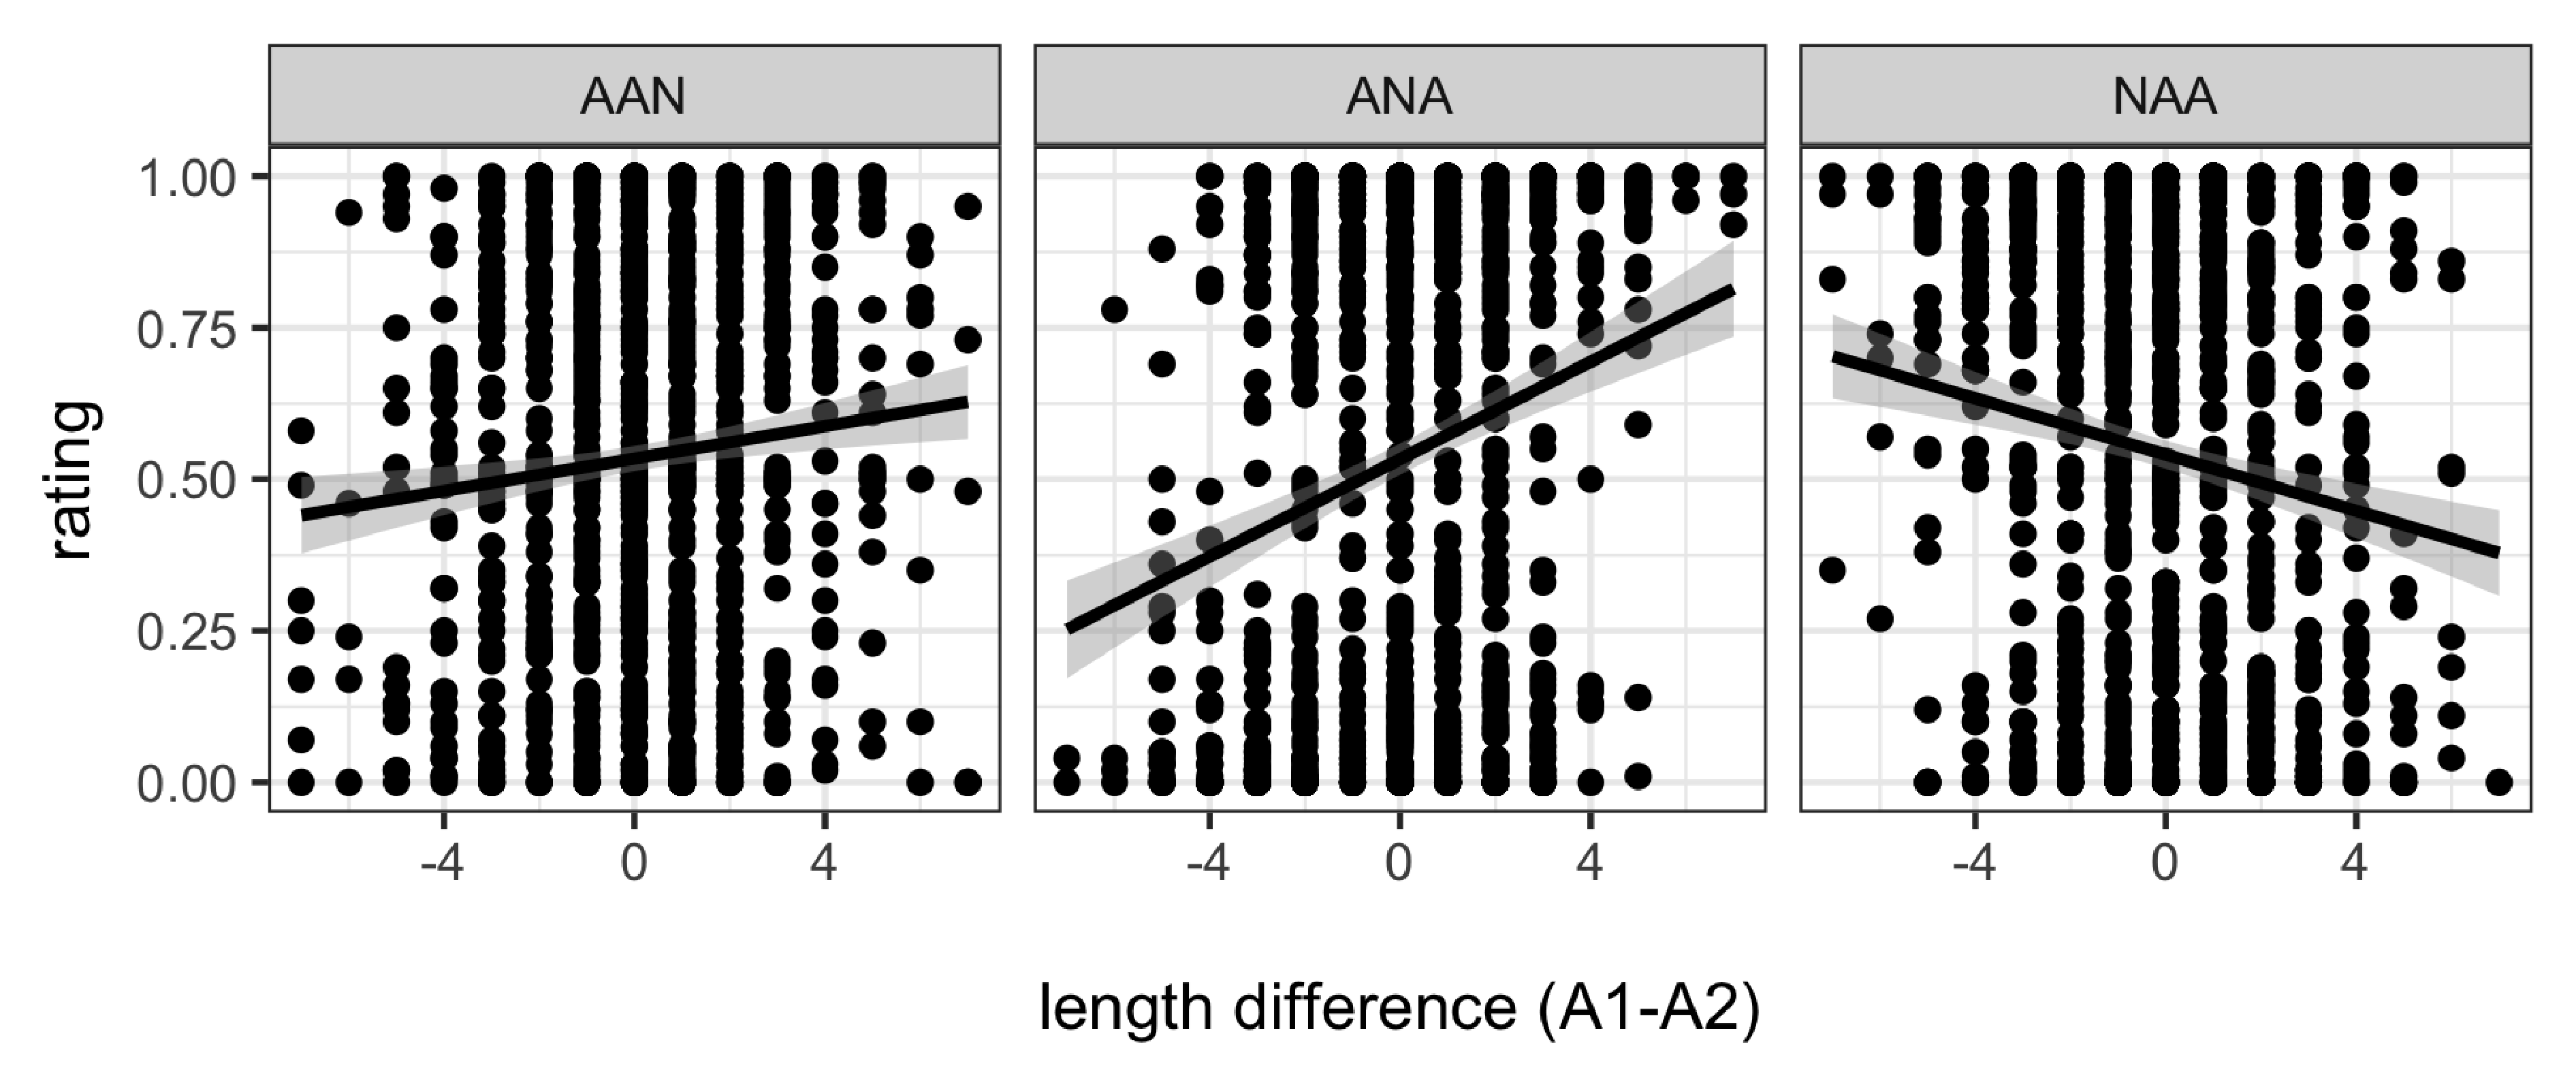
\includegraphics[width=.82\textwidth]{length.eps}
	\caption{Length difference (in characters) between the linearly-first adjective (A$_1$) and the lineary-second adjective (A$_2$) for a multi-adjective nominal, plotted against the slider rating for that nominal. In AAN and ANA, longer adjectives are preferred earlier; in NAA, longer adjectives are preferred later.}
	\label{length}
\end{figure}

\begin{figure}[h]
	\centering
	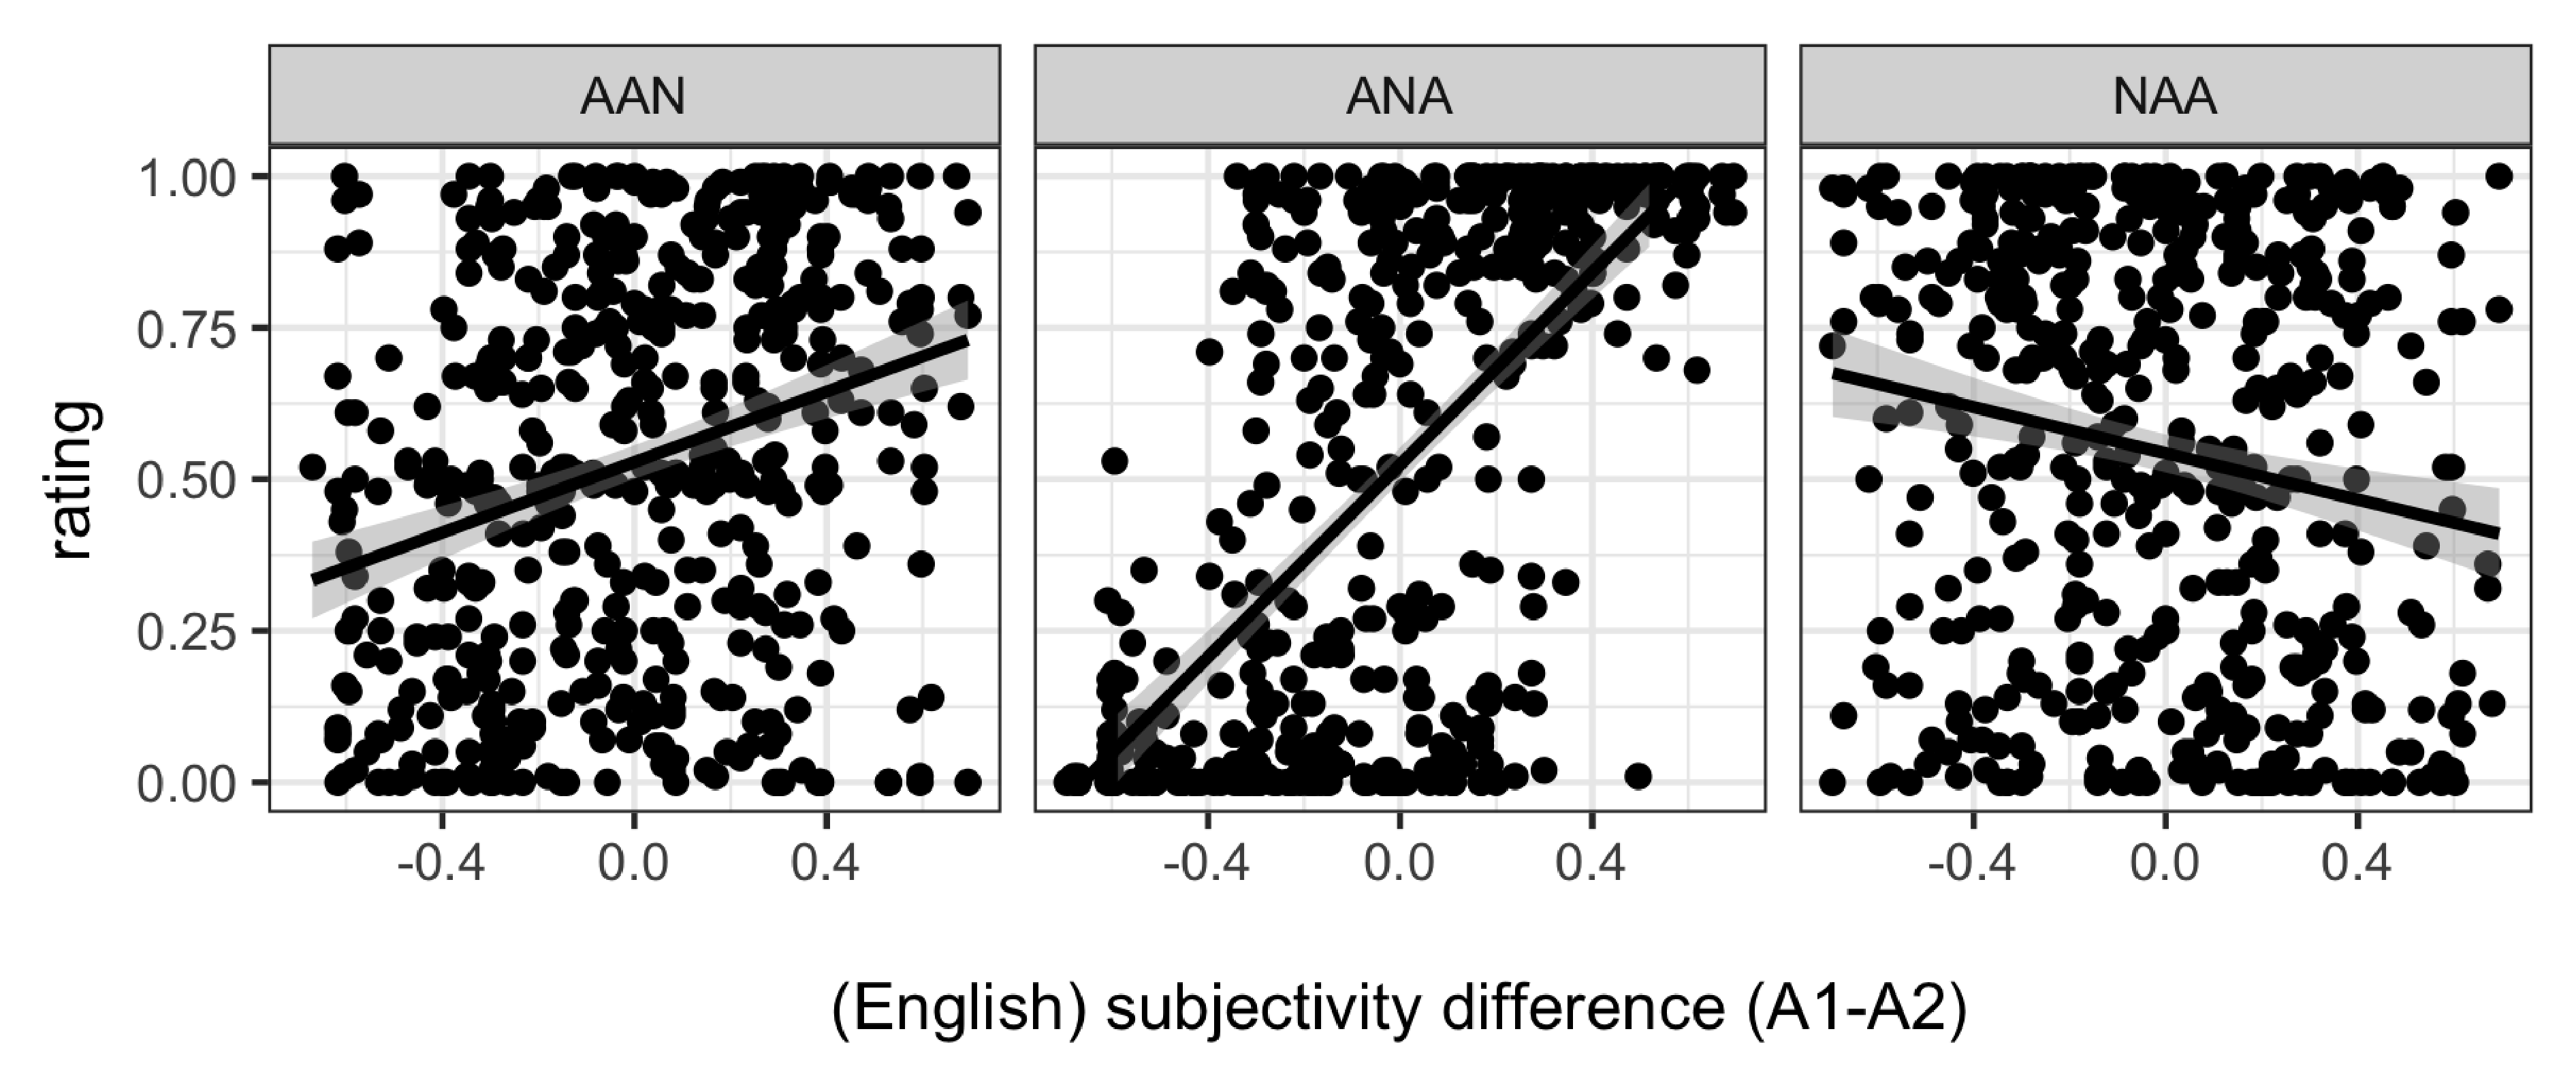
\includegraphics[width=.82\textwidth]{subjectivity.eps}
	\caption{Subjectivity difference (calculated from subjectivity scores for the English translations obtained by \citealp{futrelletal2020} and \citealp{dyeretal2023}) between the linearly-first adjective (A$_1$) and the lineary-second adjective (A$_2$) for a multi-adjective nominal, plotted against the slider rating for that nominal. In AAN and ANA, adjectives with higher subjectivity are preferred earlier; in NAA, adjectives with higher subjectivity are preferred later.}
	\label{subjectivity}
\end{figure}


\begin{figure}[h]
	\centering
	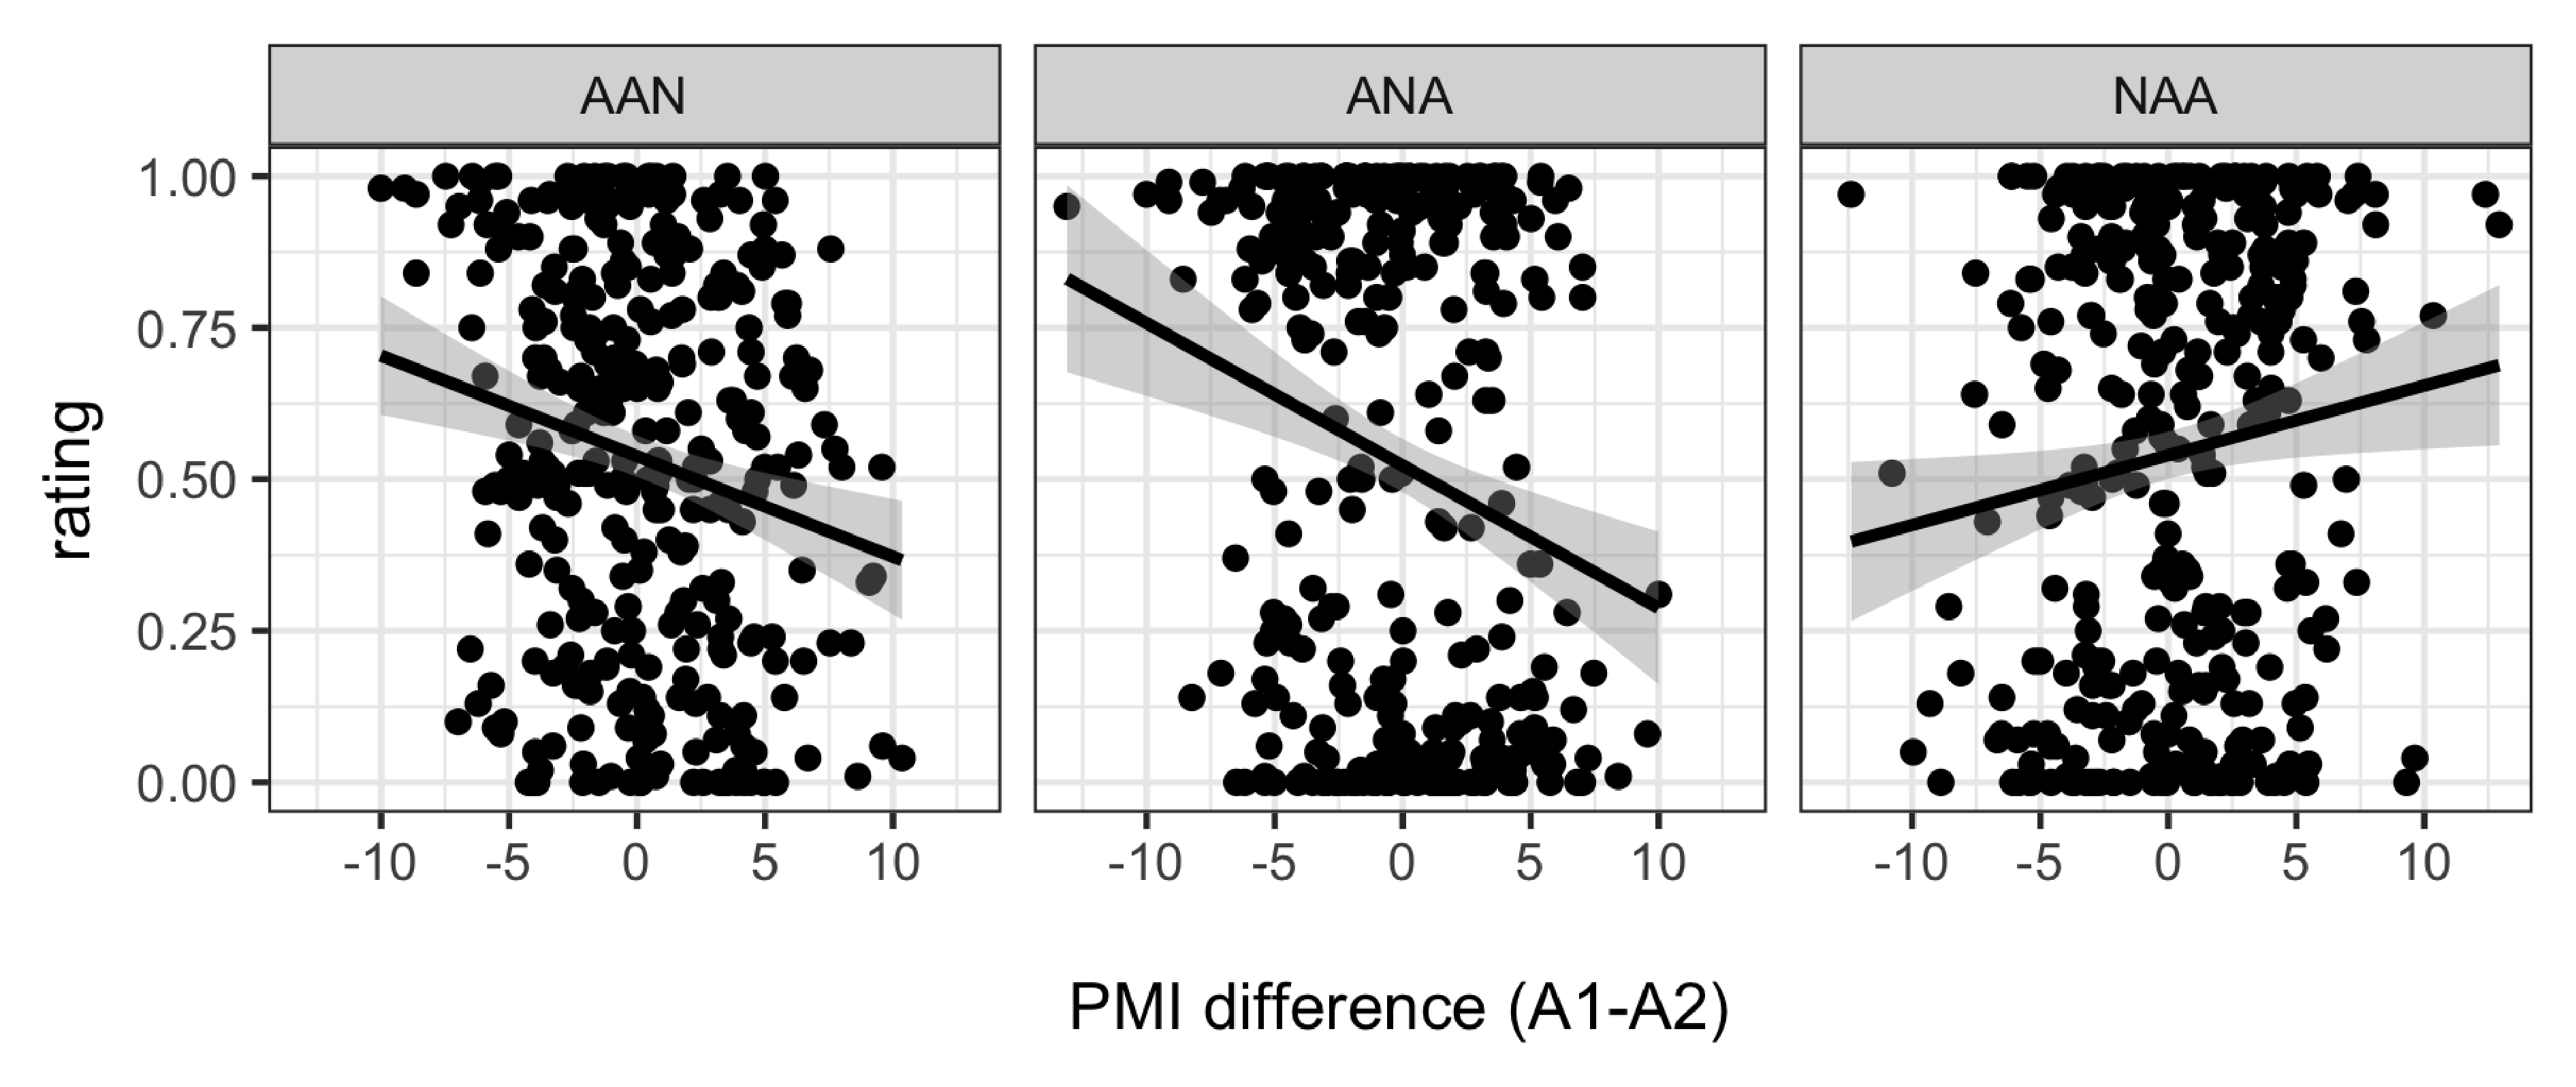
\includegraphics[width=.82\textwidth]{PMI.eps}
	\caption{PMI difference (calculated from the automatically parsed Wikipedia dump datasets released as part of the CoNLL 2017 Shared Task; \citealp{zemanetal2017}) between the linearly-first adjective (A$_1$) and the lineary-second adjective (A$_2$) for a multi-adjective nominal, plotted against the slider rating for that nominal. In AAN and ANA, adjectives with higher PMI are preferred later; in NAA, adjectives with higher PMI are preferred earlier.}
	\label{PMI}
\end{figure}




\subsection{Experiment 2: Between-subjects design}

To address the worry that our within-subjects design may have led to the absence of stable preferences for NAA ordering because of the salient ANA template alternative, we ran a follow-up experiment with a between-subjects design. In this new version, participants were randomly assigned to one of the three templates and encountered all multi-adjective nominals in that template; the other aspects of the design remain  unchanged.

We recruited 120 participant who did not take part in the first experiment via Prolific.com. As before, we restricted our sample to people who indicated that they were raised monolingually speaking Italian. Of the 120 participants recruited, 110 indicated only Italian as the language spoken at home when they were children; we include their data in the results reported below.
 
Figure \ref{results} plots preferred-distance measures grouped by adjective semantic class. We find essentially the same pattern of results from the within-subjects design; to the extent that anything differs, we observed even stronger preferences in the ANA template in the between-subjects design.


\section{Discussion}

\cite{cinque1994, cinque2010} posits that the prenominal order is base generated, adhering to a syntactic sequence, while the postnominal order in Italian depends on the movement of the N(P) to a position to the left of (part of) the adjectival sequence. This model is consistent with our results relating to the ANA template (displaying the same hierarchy as AAN order in English). The model is not compatible with the results relating to NAA. If the theory is weakened (e.g., by introducing postnominal reduced relative clauses not subject to ordering requirements; \citealp{cinque2010}), then predictions concerning ANA are lost. 

We conclude that we cannot predict adjective ordering by imputing cross-linguistic differences to movement. This finding further suggests that adjectival hierarchies should not be built into syntactic hierarchies, but rather handled by more general communicative pressures, as suggested recently by \cite{scontrasetal2017adjectives,scontrasetal2019adjectives,futrelletal2020,dyeretal2023}, either at the semantico-pragmatic interface (e.g., via factors such as adjective subjectivity) or at the externalization interface (e.g., via factors such as length or PMI).


\section*{References}

\bibliographystyle{chicago}
\bibliography{greg}


\end{document}